\documentclass[11pt]{article}
\usepackage{amsmath, amssymb, amscd, amsthm, amsfonts}
\usepackage{graphicx}
\usepackage{hyperref}
\usepackage{subfigure}
\usepackage{float}
\usepackage{rotating}
\usepackage{tikz}
\usepackage{xcolor}
\usepackage{listings}
\usepackage{ltablex}

\usepackage{longtable}
\definecolor{vgreen}{RGB}{104,180,104}
\definecolor{vblue}{RGB}{49,49,255}
\definecolor{vorange}{RGB}{255,143,102}
\lstdefinestyle{verilog-style}
{
    language=Verilog,
    basicstyle=\small\ttfamily,
    keywordstyle=\color{vblue},
    identifierstyle=\color{black},
    commentstyle=\color{vgreen},
    numbers=left,
    numberstyle=\tiny\color{black},
    numbersep=10pt,
    tabsize=4,
    moredelim=*[s][\colorIndex]{[}{]},
    literate=*{:}{:}1
}

\makeatletter
\newcommand*\@lbracket{[}
\newcommand*\@rbracket{]}
\newcommand*\@colon{:}
\newcommand*\colorIndex{%
    \edef\@temp{\the\lst@token}%
    \ifx\@temp\@lbracket \color{black}%
    \else\ifx\@temp\@rbracket \color{black}%
    \else\ifx\@temp\@colon \color{black}%
    \else \color{vorange}%
    \fi\fi\fi
}
\makeatother

\usepackage{trace}



\oddsidemargin 0pt
\evensidemargin 0pt
\marginparwidth 40pt
\marginparsep 10pt
\topmargin -20pt
\headsep 10pt
\textheight 8.7in
\textwidth 6.65in
\linespread{1.2}

\title{Digital Bubble Level - Cell Layout}
\author{Vladislav Pomogaev - 26951160}
\date{December 5, 2021}

\newcommand{\rr}{\mathbb{R}}

\newcommand{\al}{\alpha}
\DeclareMathOperator{\conv}{conv}
\DeclareMathOperator{\aff}{aff}

\begin{document}

\maketitle

\section{Introduction}
This device forms a digital bubble level; also called a spirit level. It can be helpful in levelling things horizontally. The project began as a synthesised set of Verilog files for the Efinix Xyloni FPGA development board, but I have since extracted the core FSM from that project, laid it out with the 45nm standard cell library, and verified its operation though simulations.
\begin{figure}[H]
    \centering
    \subfigure[]{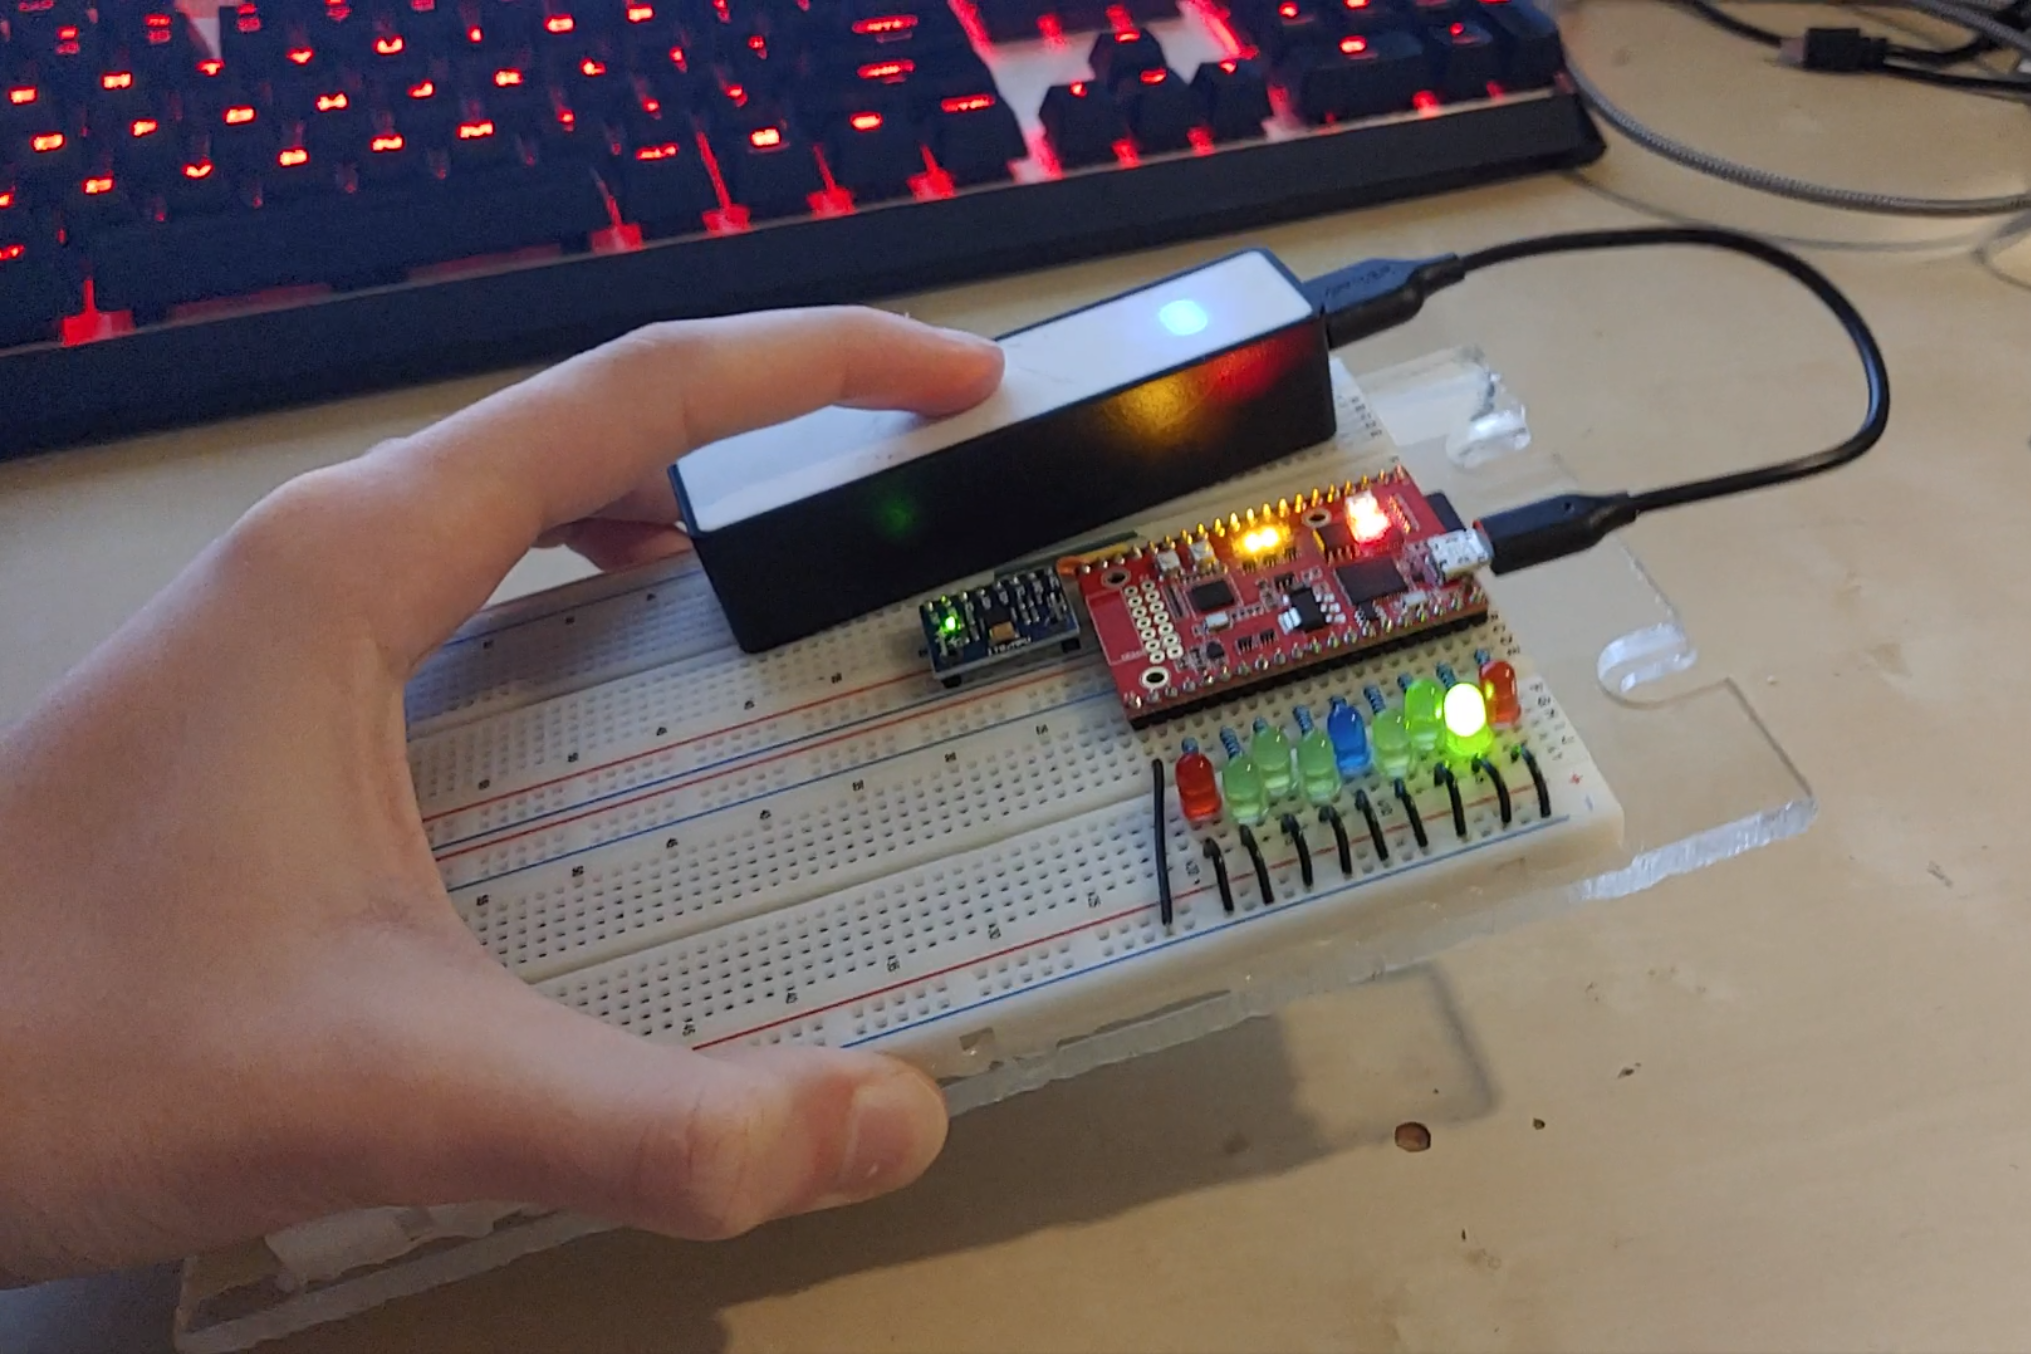
\includegraphics[width=0.32\textwidth]{tilt_1.png}} 
    \subfigure[]{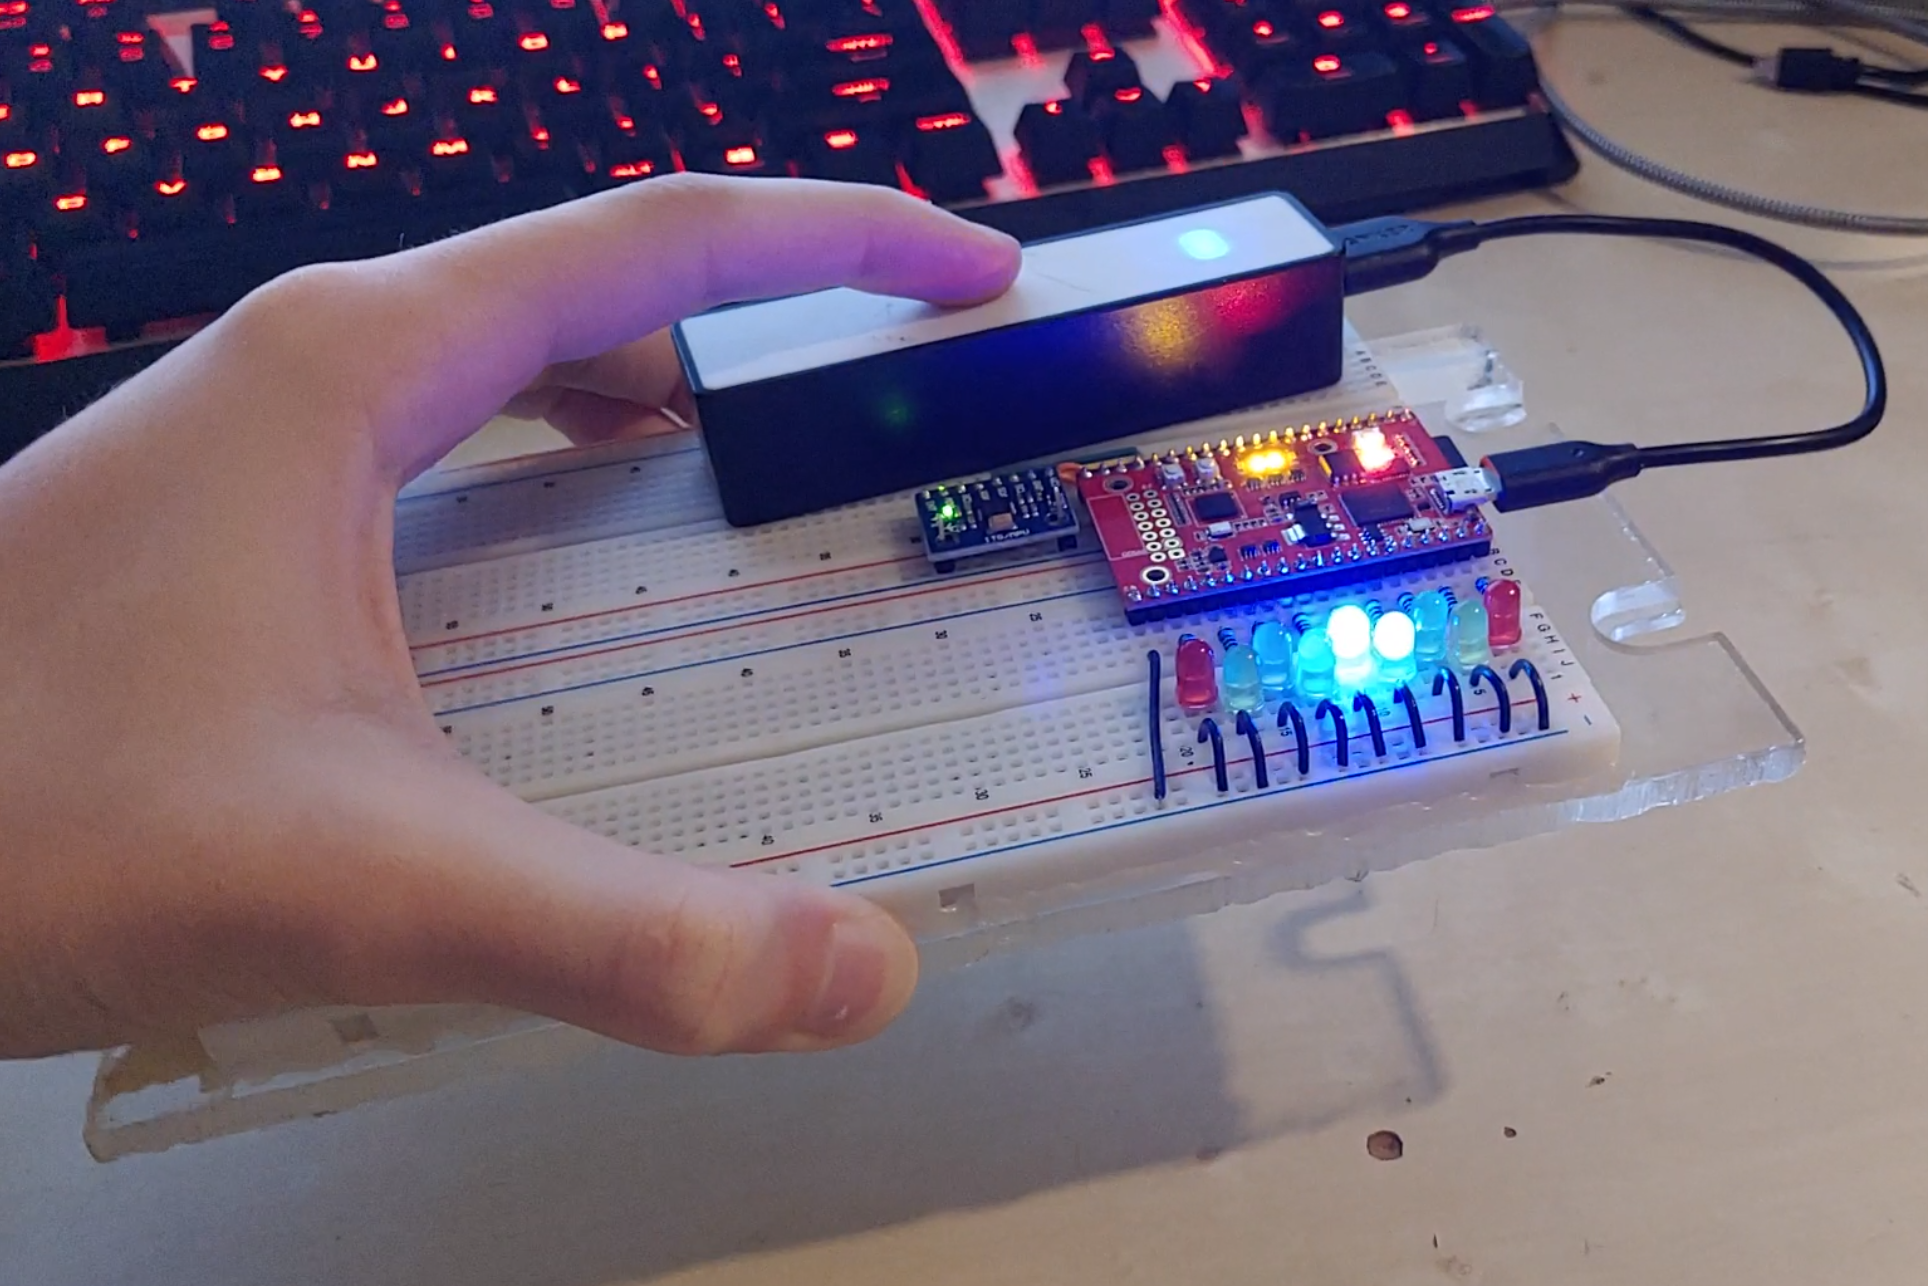
\includegraphics[width=0.32\textwidth]{tilt_3.png}} 
    \subfigure[]{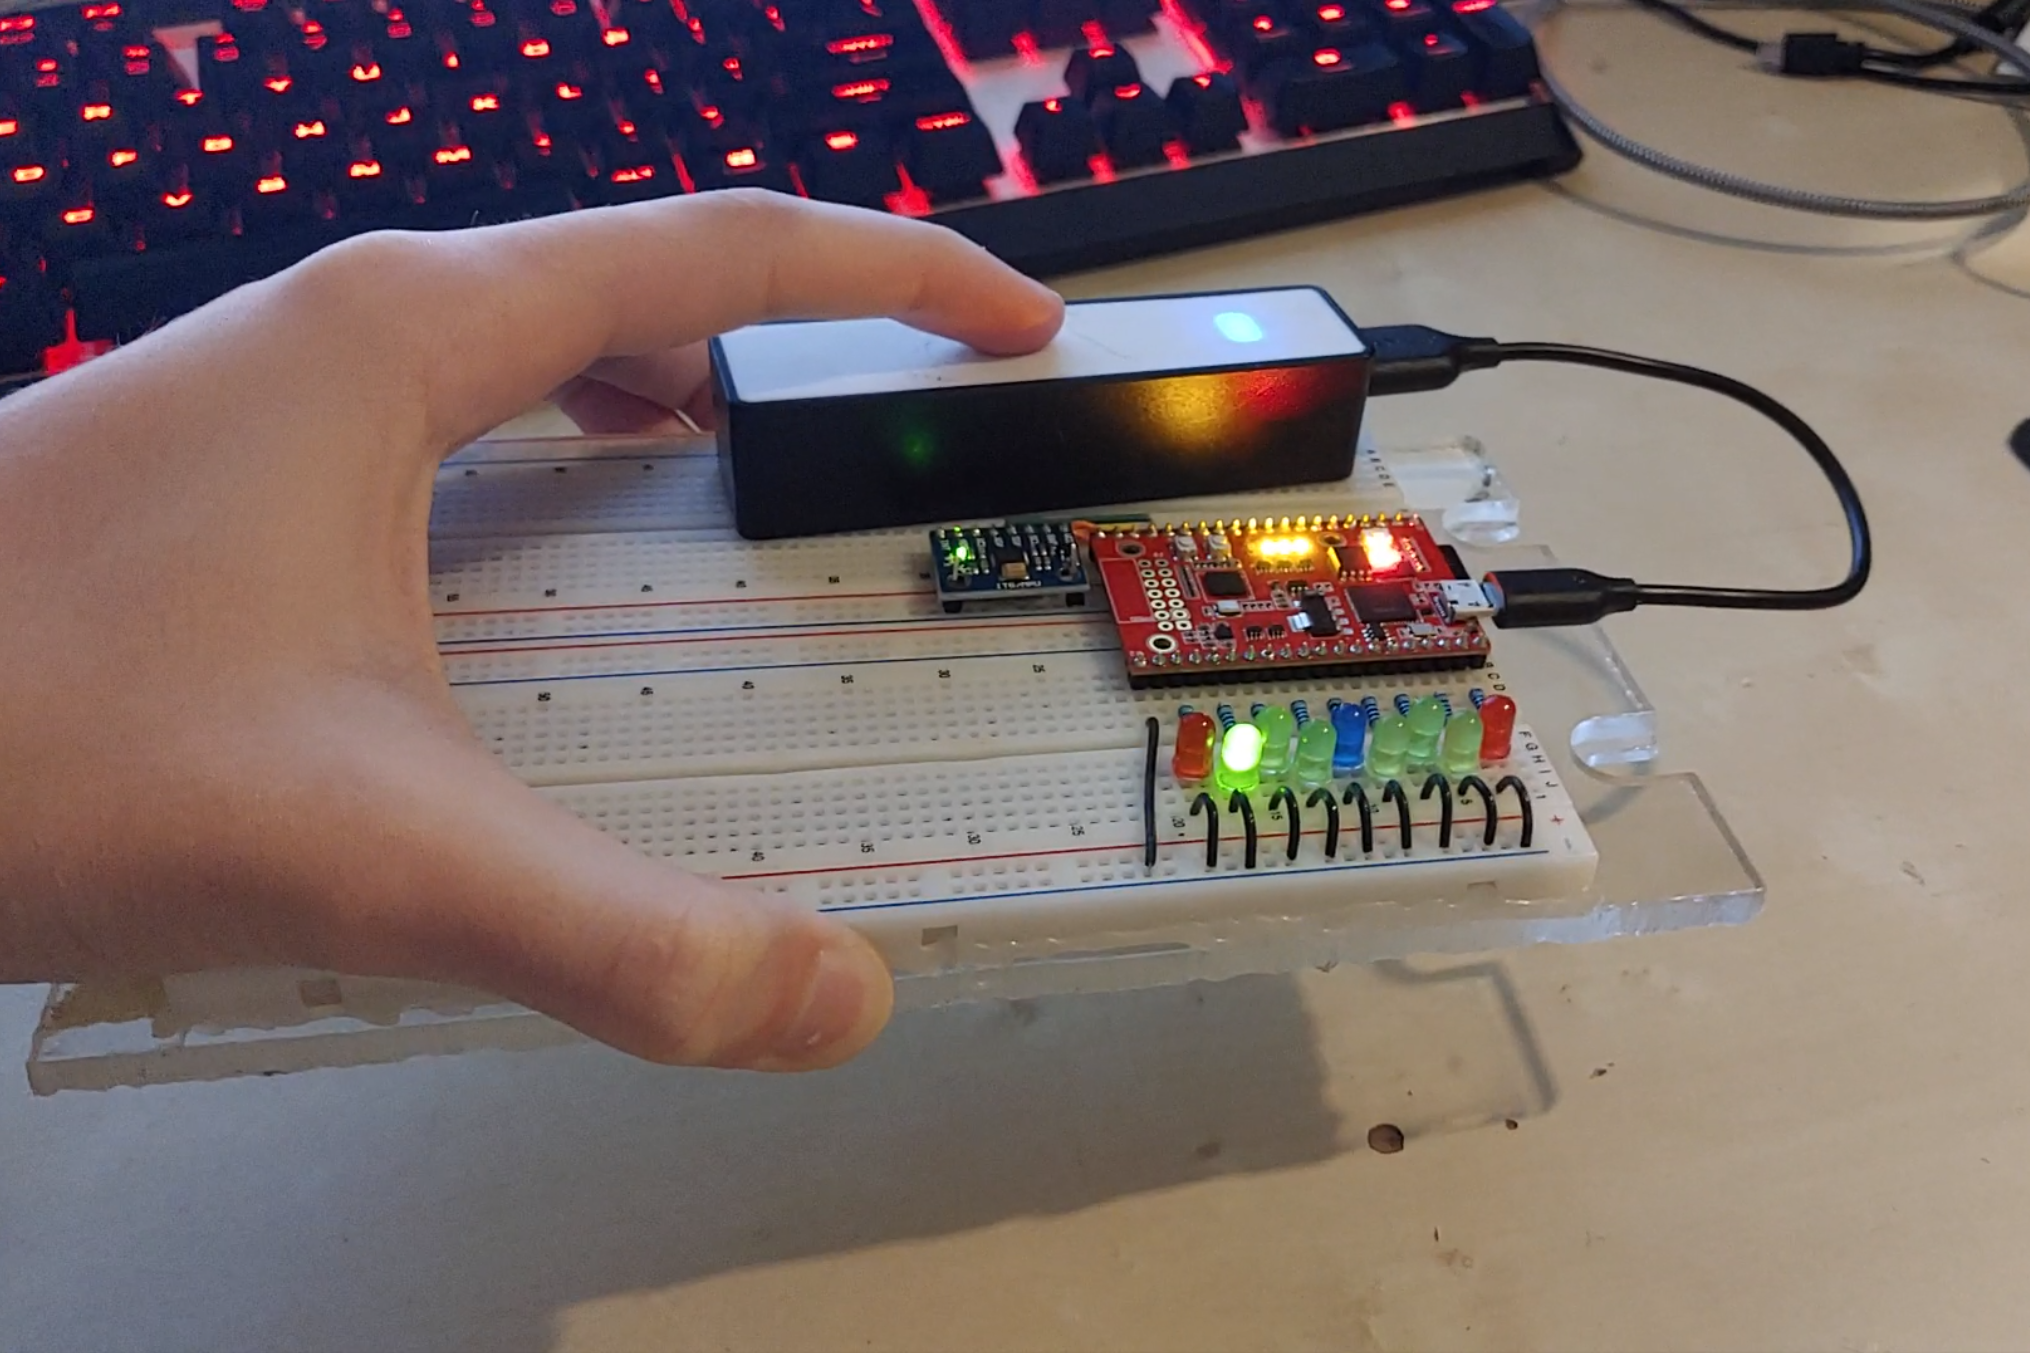
\includegraphics[width=0.32\textwidth]{tilt_2.png}}
    \caption{Photo stills of the original device in action. When you tilt the device to the left as in a), the LEDs to the right light up. As you tilt the device more to the right, the lit LED moves from right to left as in b) and c). When level, the blue center LED lights up.}
\end{figure}

\section{Overview}
\begin{figure}[H]
    \centering
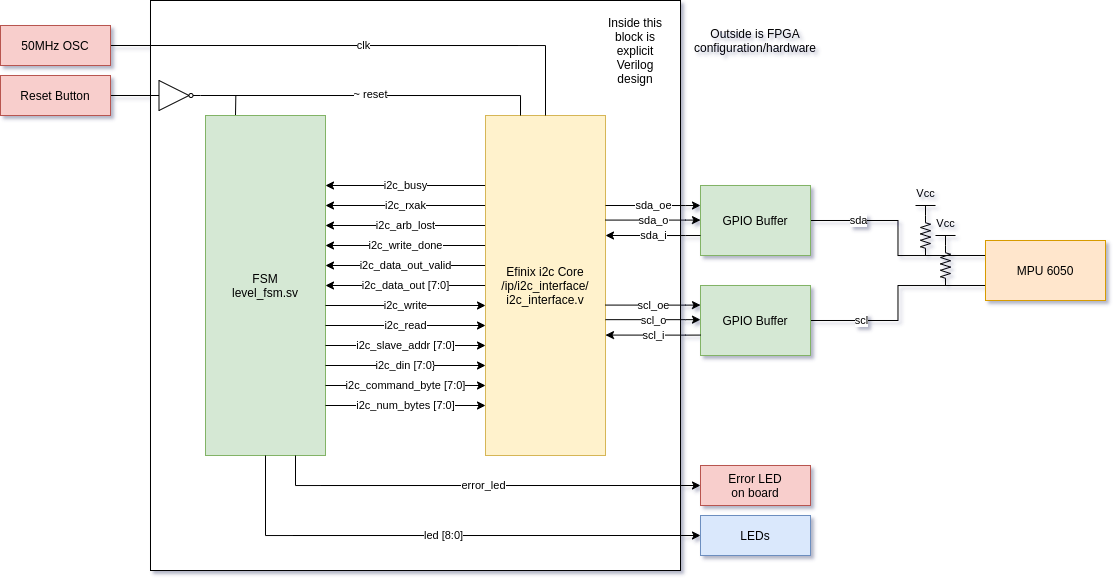
\includegraphics[width=0.99\textwidth]{fsm.png}
    \caption{Block diagram of the FSM and how it forms the bubble-level system. The level FSM talks to the I2C core, which communicates to the MPU via a set of buffered GPIO blocks on the FPGA. A reset button resets all FSMs to their initial state. The design runs is compiled for a 50MHz clock constraint. The output to outside of the FPGA is buffered through the GPIO logic blocks, which was the reason I used IP specific to the FPGA. I only did the layout and verification for the level\_fsm.sv file from the original project.}
\end{figure}


\subsection{Ports}

% Please add the following required packages to your document preamble:
% \usepackage{graphicx}
\begin{table}[H]
\resizebox{\textwidth}{!}{%
\begin{tabular}{llllll}
Port & Width (bits) & Interface & Direction & Description &  \\
clk\_i & 1 & System & Input & Clock input. 50MHz max. &  \\
reset\_i & 1 & System & Input & Active high reset input &  \\
i2c\_busy\_i & 1 & I2C & Input & Logic high indicates that the I2C bus is busy. &  \\
i2c\_rxak\_i & 1 & I2C & Input & Logic low indicates that the I2C slave device received and acknowledged the I2C transfer &  \\
i2c\_arb\_lost\_i & 1 & I2C & Input & Logic high indicated there is arbitration lost in the I2C transfer &  \\
i2c\_write\_done\_i & 1 & I2C & Input & Logic high indicates that I2C master write data is sent and ready to accept by I2C slave device. &  \\
i2c\_data\_out\_valid\_i & 1 & I2C & Input & Logic high indicates that I2C master read data is valid and ready to read by user. &  \\
i2c\_data\_out\_i & 8 & I2C & Input & Data read input port &  \\
i2c\_write\_o & 1 & I2C & Output & Write to slave strobe high &  \\
i2c\_read\_o & 1 & I2C & Output & Read from slave strobe high &  \\
i2c\_slave\_addr\_o & 8 & I2C & Output & Address of slave in 8bit format. Add trailing zero to use 7-bit addressing. &  \\
i2c\_din\_o & 8 & I2C & Output & Data read from slave &  \\
i2c\_command\_byte\_o & 8 & I2C & Output & Command byte sent to slave. (Register to read from) &  \\
i2c\_num\_bytes\_o & 8 & I2C & Output & Number of bytes of data to write or read. Includes the command byte (if sending one byte, i2c\_num\_bytes\_o = 'd2) &  \\
error\_led\_o & 1 & System & Output & Active high if an error has occured in state machine; lost bytes, error writing to slave or reading. Reset FSM to try again. &  \\
led\_o & 9 & System & Output & LED array output of bubble level & 
\end{tabular}%
}
\end{table}

\section{Standard Library Layout}

\begin{figure}[H]
    \centering
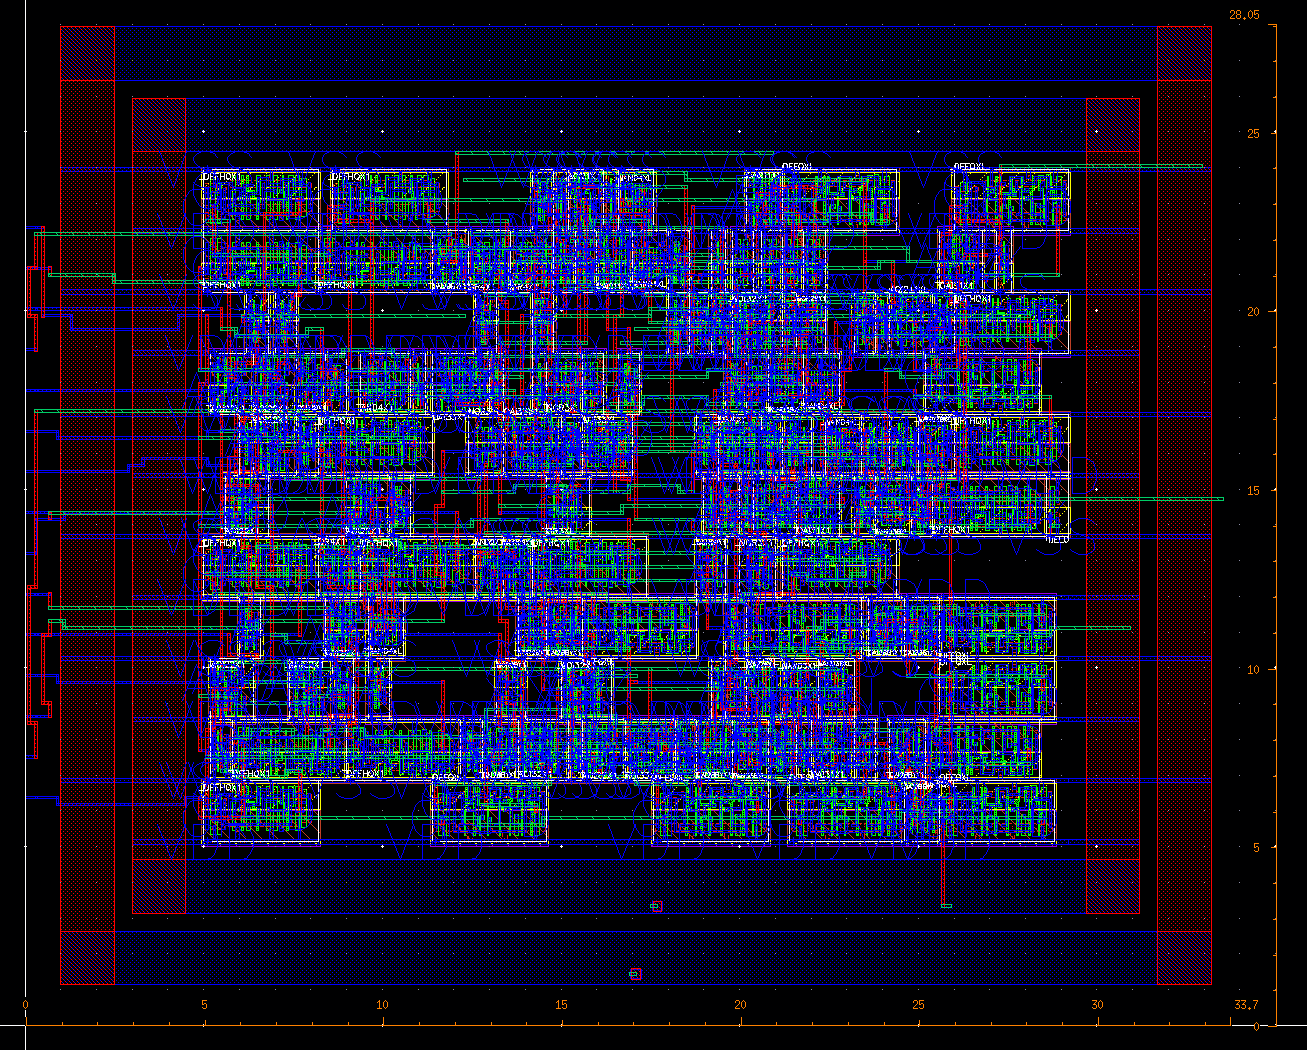
\includegraphics[width=0.99\textwidth]{layout2.png}
    \caption{The level\_fsm.sv file was synthesized and laid out using the 45nm standard cell library provided. The ports were aligned as such: inputs on the left, outputs on the right, and power on the bottom. The very outer dimensions are 33um x 28um, for a total area of 924um\^2.}
\end{figure}


\section{Simulation/Verification}

\begin{figure}[H]
    \centering
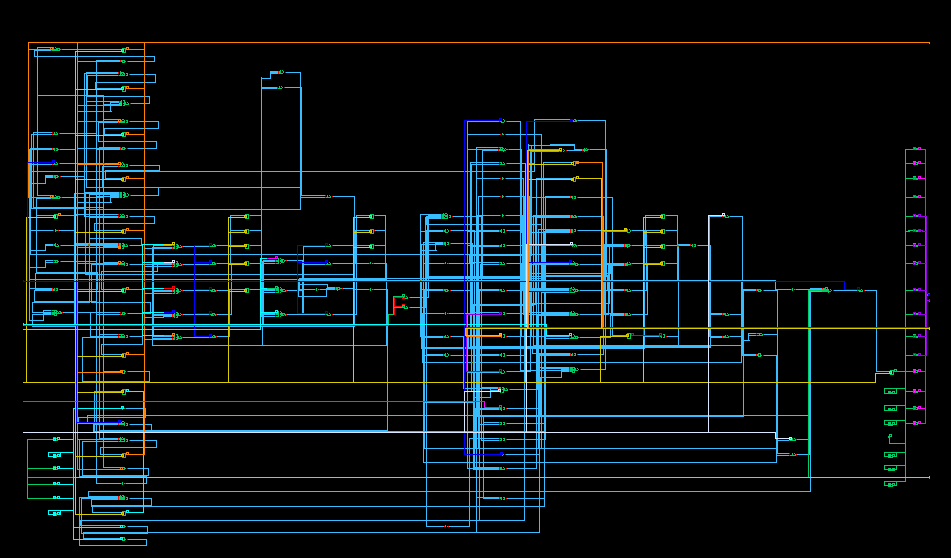
\includegraphics[width=0.99\textwidth]{schem3.png}
    \caption{The Verilog file was also translated to a RTL layout and displayed in viewable form. Here we see the entire FSM schematic in terms of logic gates.}
\end{figure}


\begin{figure}[H]
    \centering
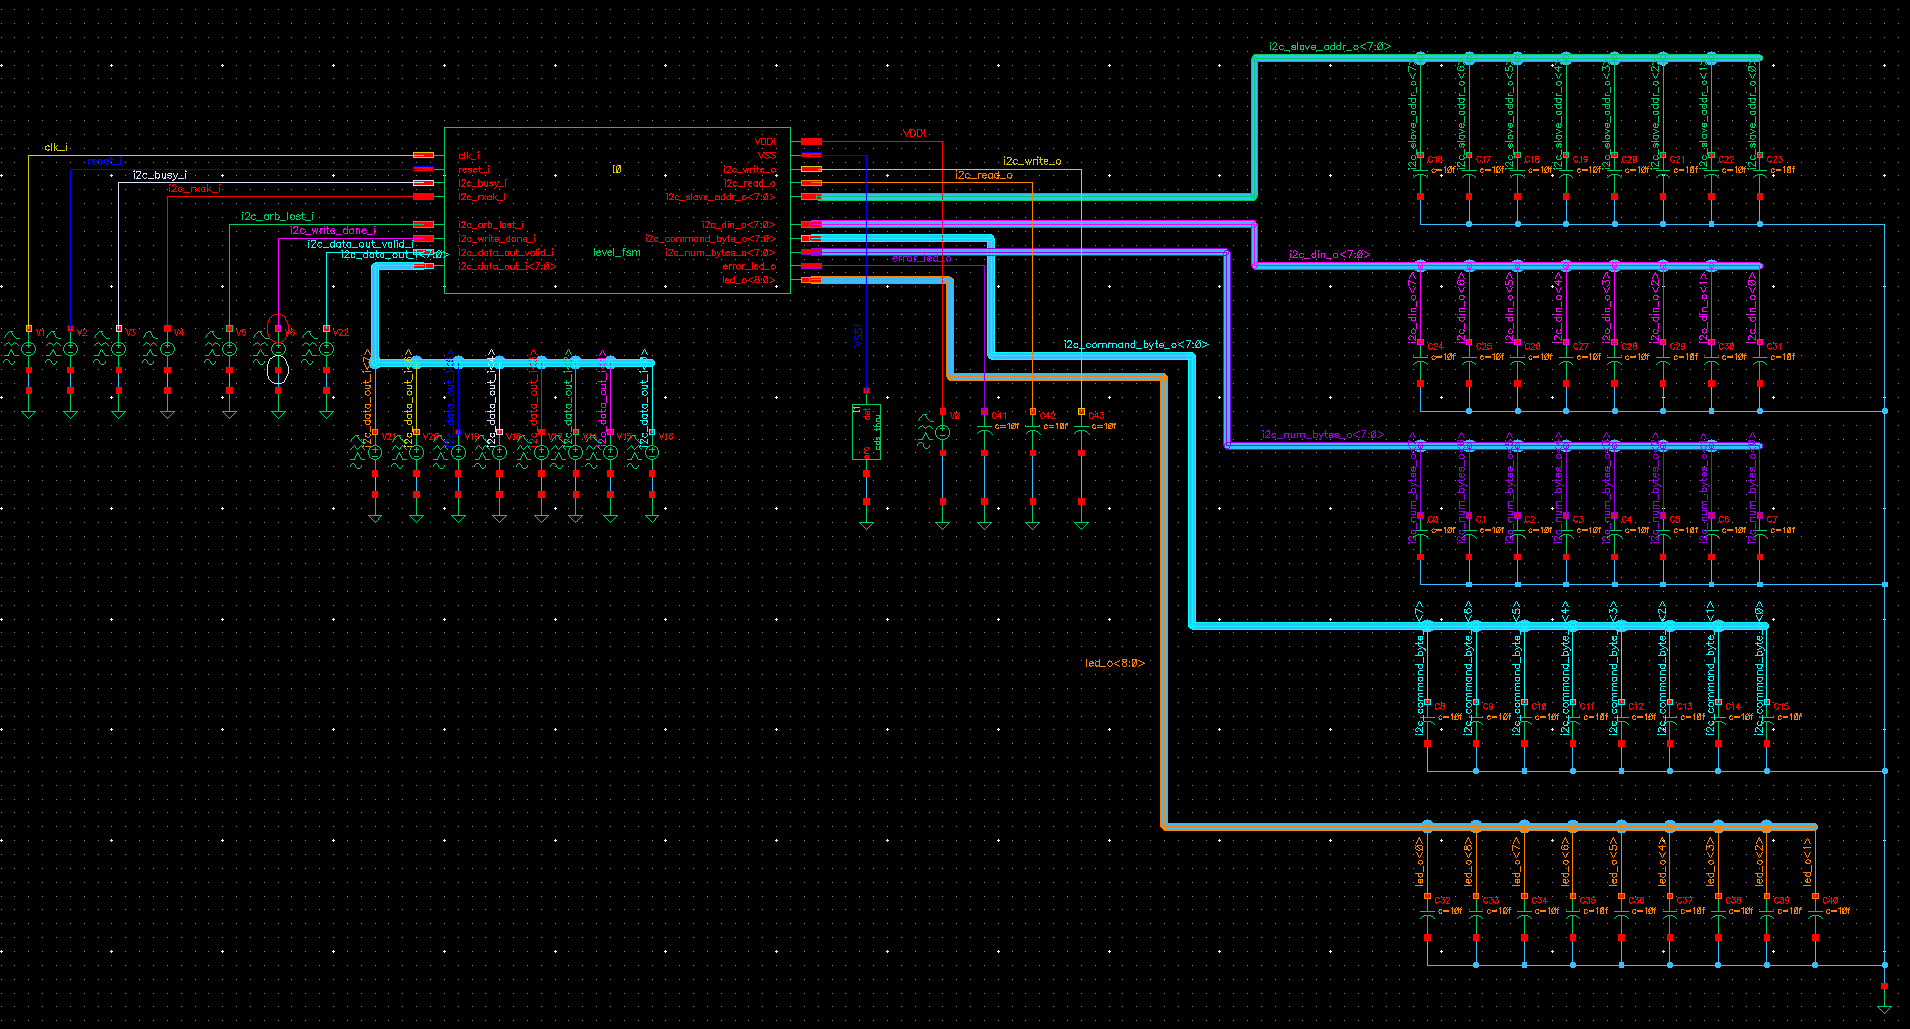
\includegraphics[width=0.99\textwidth]{schem2.png}
    \caption{The previous RTL design was transformed into a new cell view. This cell view was placed in a test-bench schematic. Each output of the FSM was loaded with a 10fF capacitor. An array of 1V supplies was used to drive the input signals.}
\end{figure}


\begin{figure}[H]
    \centering
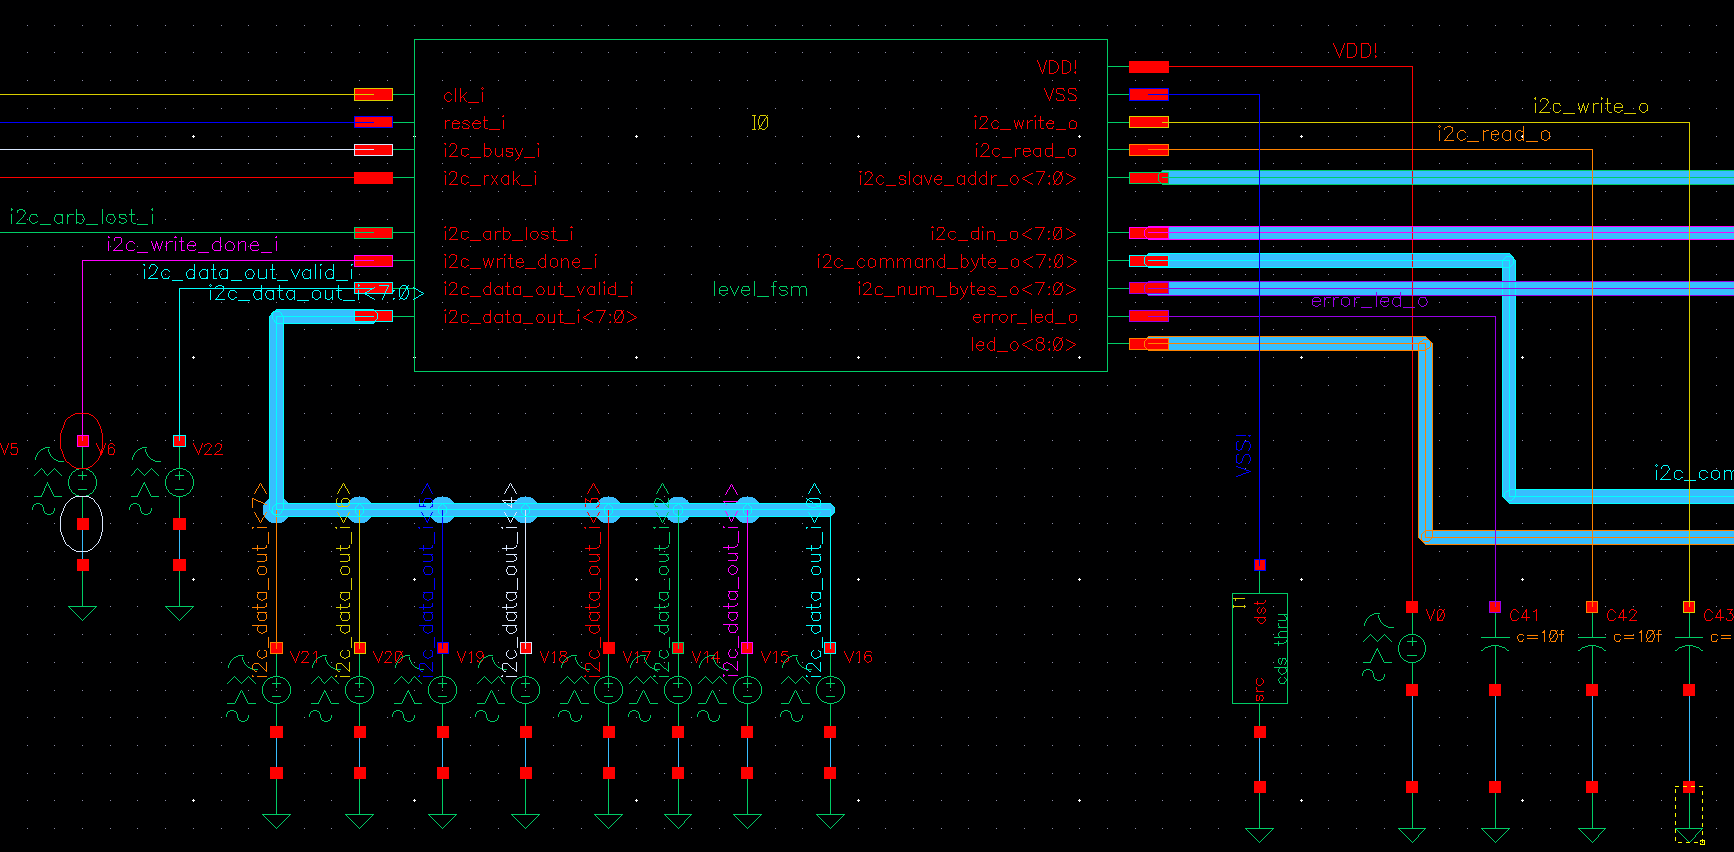
\includegraphics[width=0.99\textwidth]{closeup1.png}
    \caption{Here is a closeup of the test-bench schematic. The voltage input signals were set up manually using an array of input voltage levels that corresponded to the input vectors used in the original Verilog test bench.}
\end{figure}



\begin{figure}[H]
    \centering
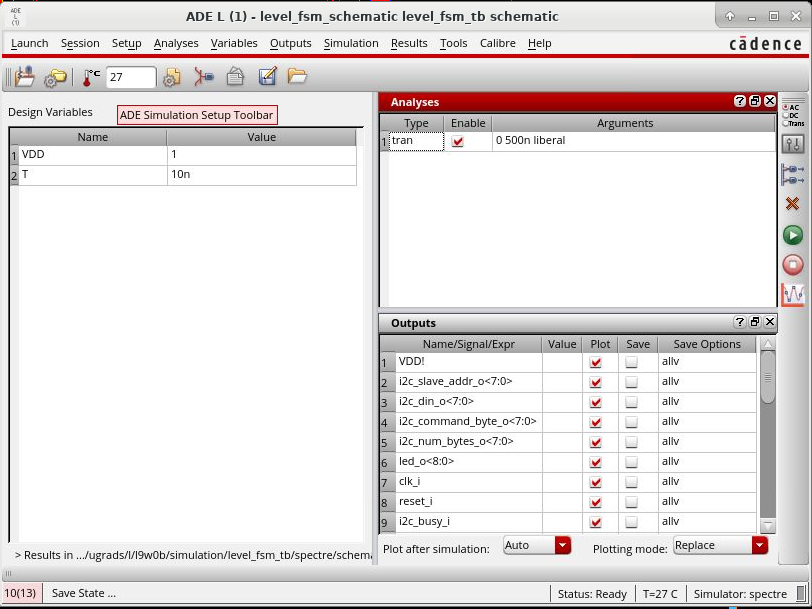
\includegraphics[width=0.99\textwidth]{simsetup.png}
    \caption{The simulation was set up using ADE. The simulation duration was the same length as the original Verilog test bench file.}
\end{figure}
\pagebreak


\begin{figure}[H]
    \centering
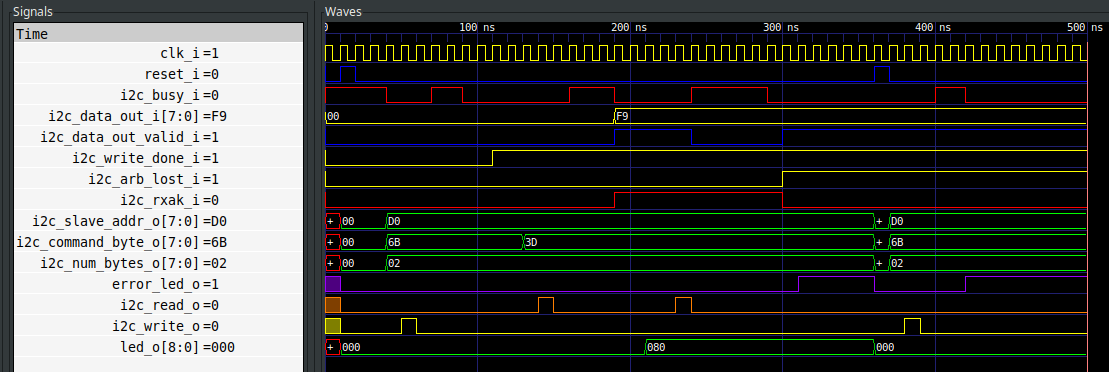
\includegraphics[width=0.99\textwidth]{verilogtb.png}
    \caption{For comparison, here is the input and output vector of the original Verilog simulation. This simulation tests does the following in this order: 1) FSM reset 2) Write to accelerometer to wake it up 3) Wait for valid response 4) Read from accelerometer register 5) Display level on LEDs. 6) Read from accelerometer register, but this time receive an error 7) Verify error\_led output 8) Reset FSM 9) Write to accelerometer to wake it up, but this time receive an error 10) Verify error\_led output 11) Stall forever. This procedure tests an overwhelming majority of the FSM.}
\end{figure}

\begin{figure}[H]
    \centering
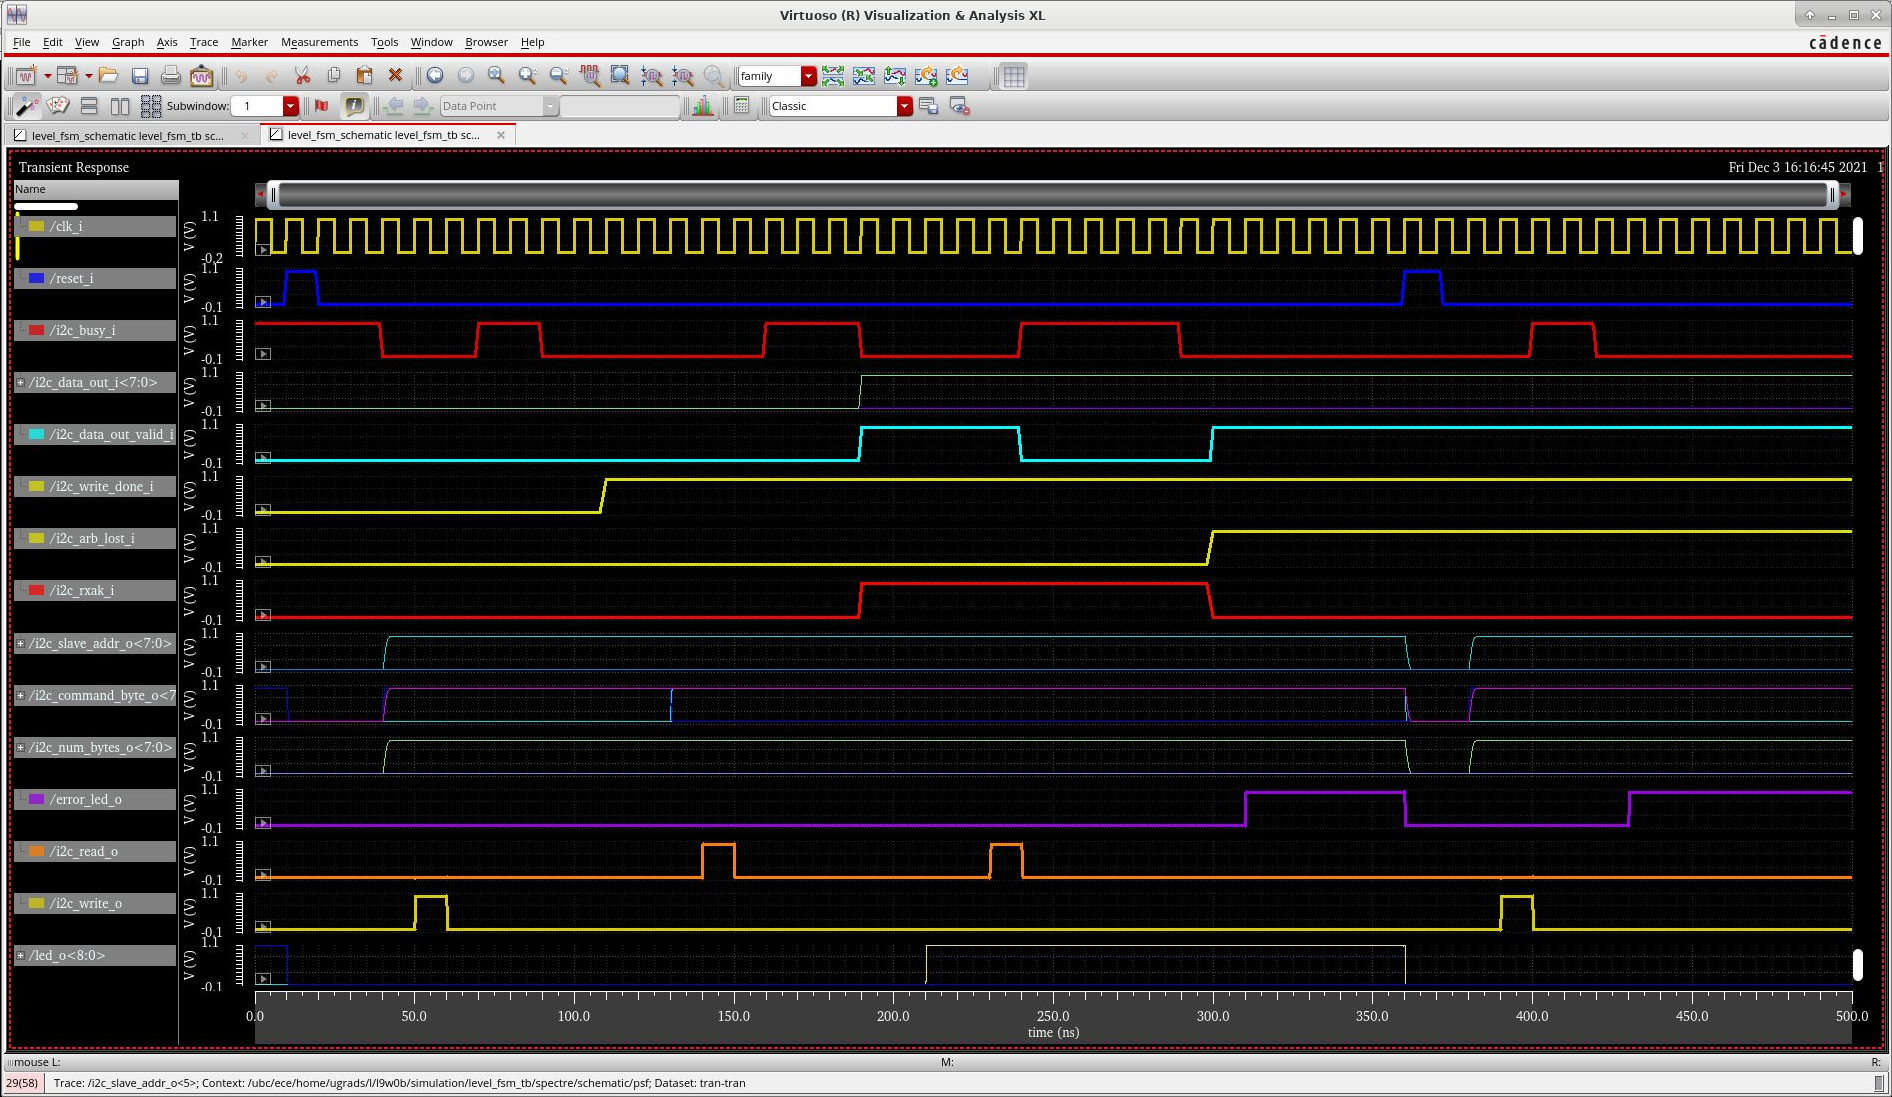
\includegraphics[width=0.99\textwidth]{waveforms.png}
    \caption{Here is the same test bench but now it is executed in Virtuoso. As we can see the waveforms are the same, but we see characteristic RC delays. The multi-bit vector values were the same in both cases. Rise time for input signals was 2ns. The layout passed the test!}
\end{figure}


\begin{figure}[H]
    \centering
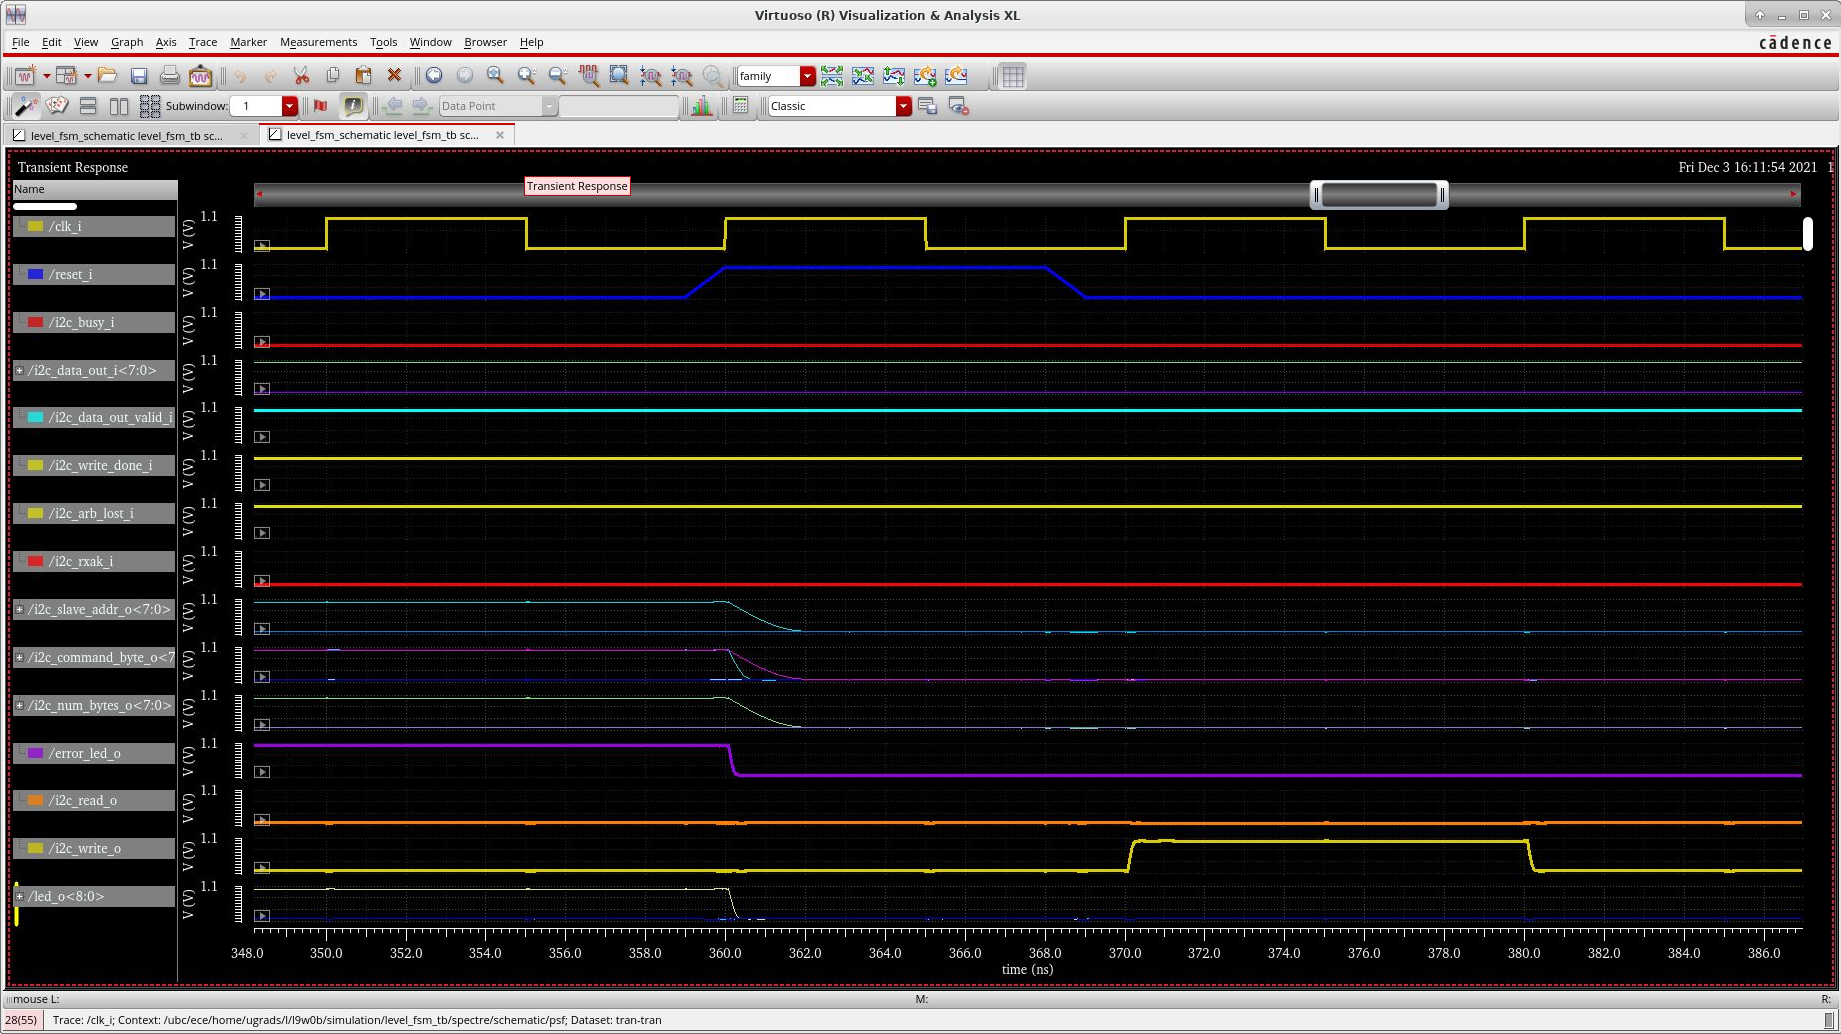
\includegraphics[width=0.99\textwidth]{disc1.png}
    \caption{I encountered an interesting problem while troubleshooting the simulation. Part of my vectors from the Verilog and Virtuoso simulations were not lining up. Upon an FSM reset, the slave addr, command byte, and num bytes should be going to 0, then back to their default non-zero values after a reset. This happens on the Verilog simulation, but not on the Virtuoso one. However, the rest of the FSM's functionality would continue as normal. Without those signals though, the FSM would not read/write from the device correctly though. I found that adjusting the length of the reset signal to be slightly MORE than two cycles would solve this issue. However, the root cause of the issue is poor test bench design. It was ultimately a setup-time violation on the reset line that would cause the FSM to skip a state. }
\end{figure}


\begin{figure}[H]
    \centering
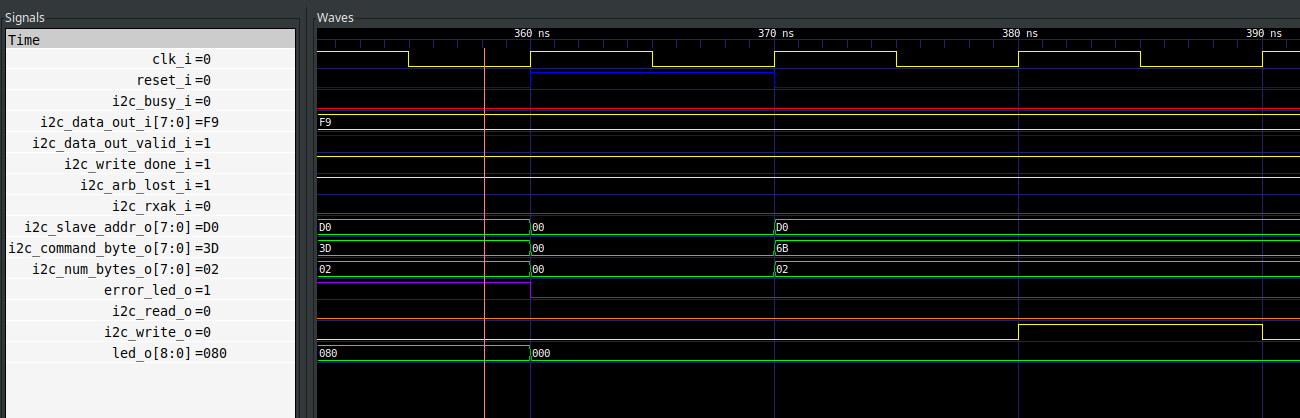
\includegraphics[width=0.99\textwidth]{disc2.png}
    \caption{What the FSM outputs should look like according to the Verilog test bench. Note how the slave address and other busses change their values at 370ns, but in the Virtuoso they do not.}
\end{figure}


\begin{figure}[H]
    \centering
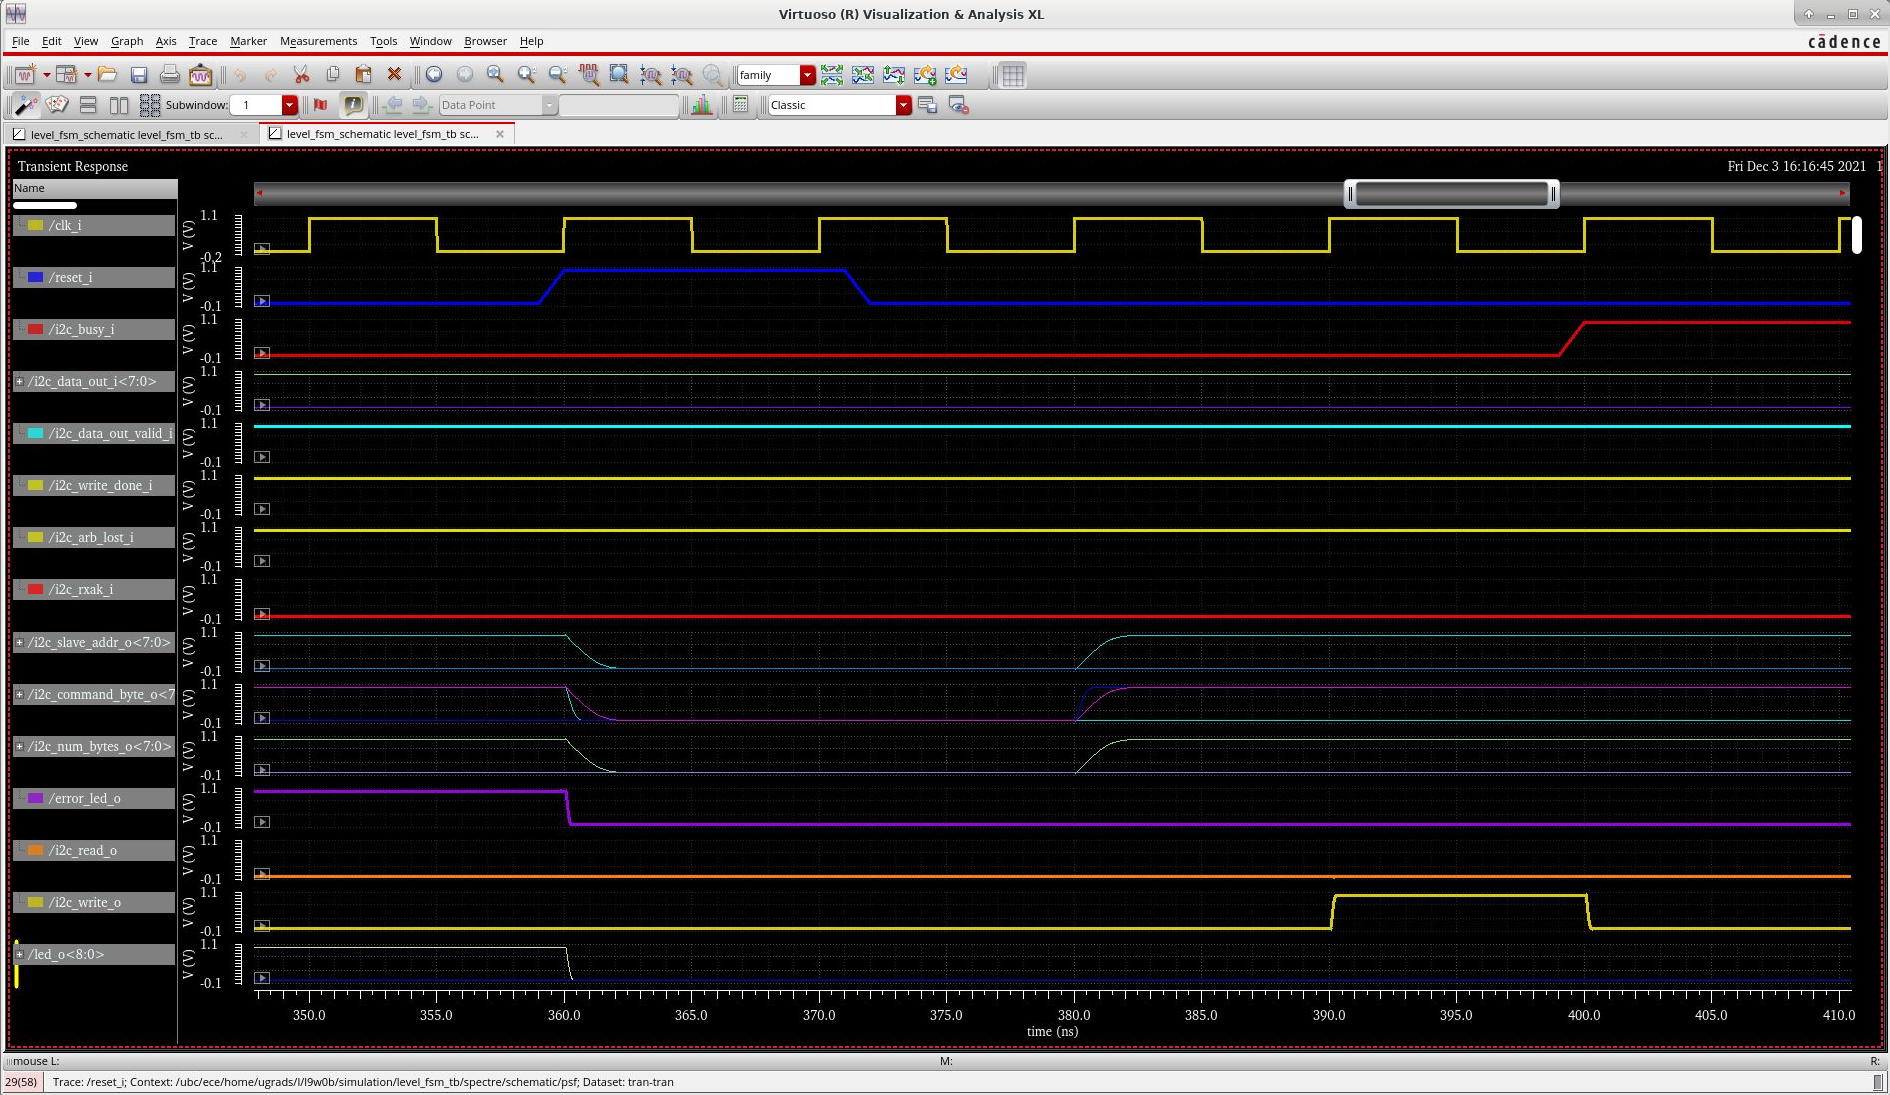
\includegraphics[width=0.99\textwidth]{fixed.png}
    \caption{Extending the reset pulse in Virtuoso solved this bug. Now the simulations are functionally identical.}
\end{figure}


\begin{figure}[H]
    \centering
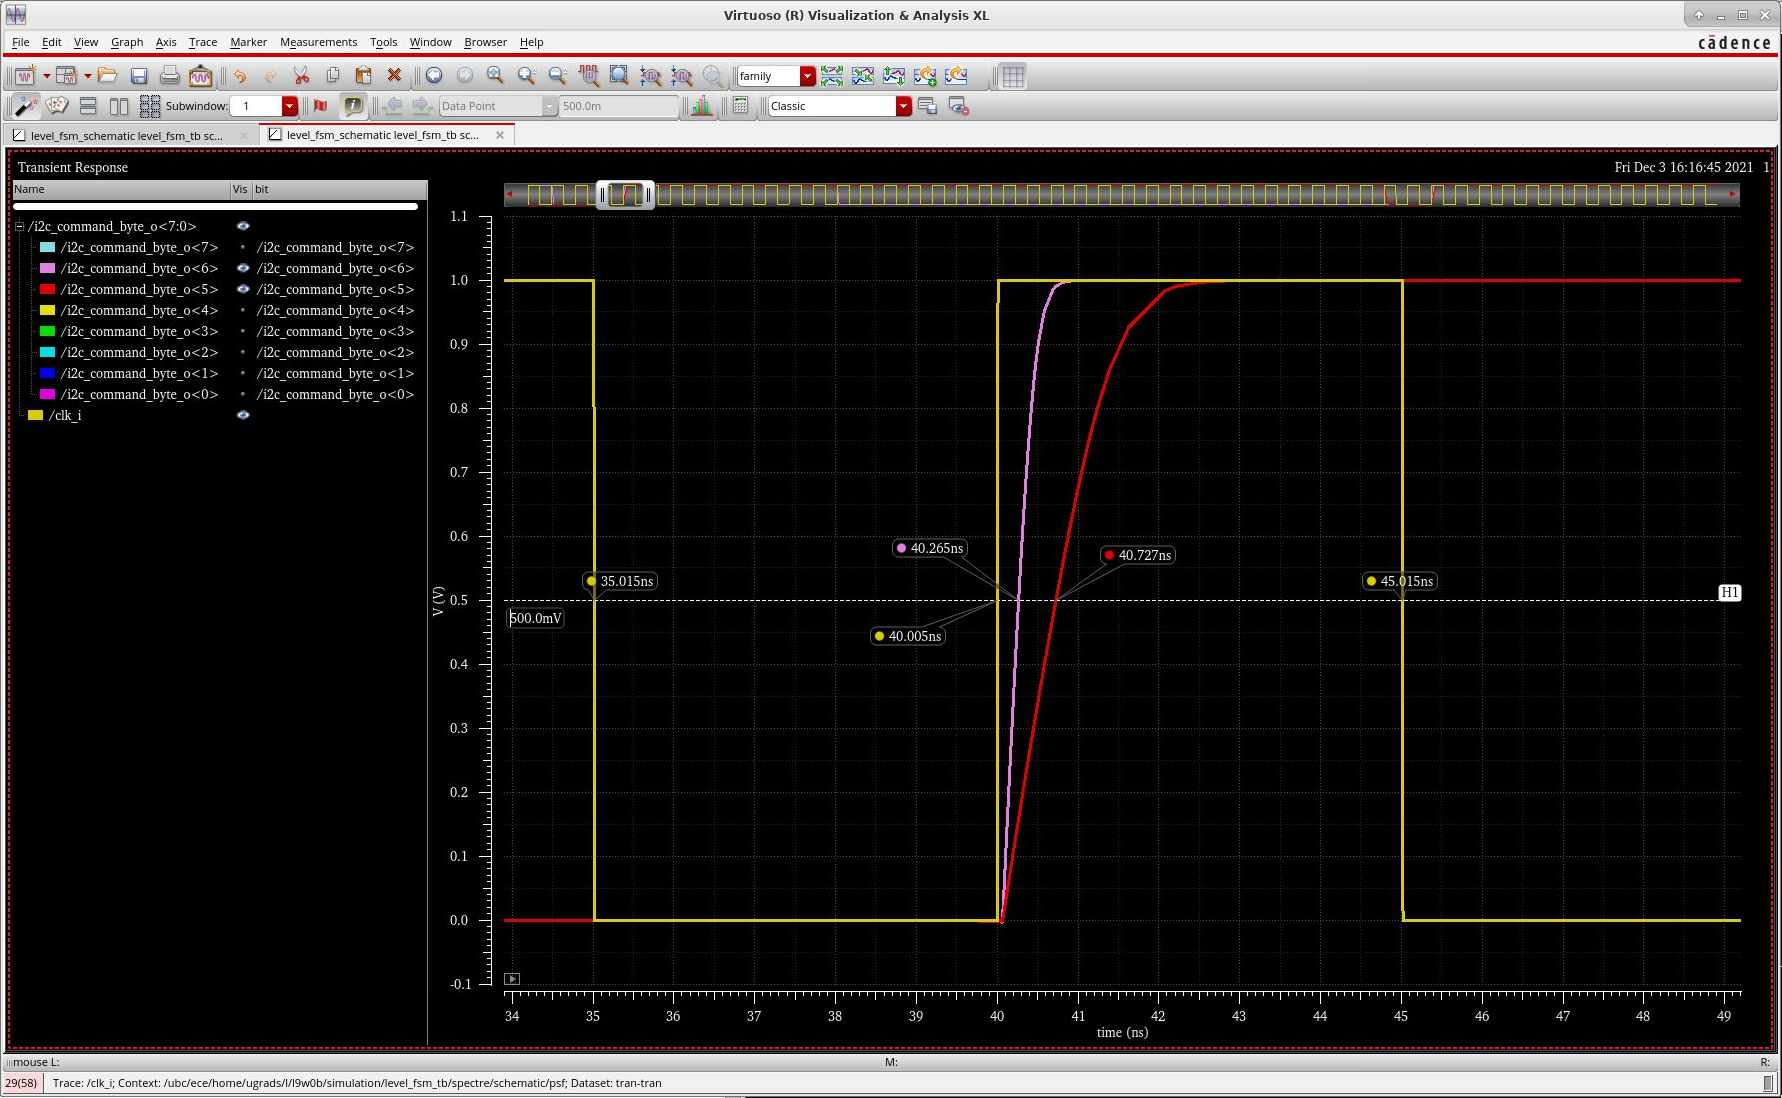
\includegraphics[width=0.99\textwidth]{delay.png}
    \caption{Another thing I played around with is measuring the propagation delay. I found the worst-case delay to be on the i2c\_command\_byte bus. The worst case delay was a staggering 722ps. Since the FSM is rather simple and it's function is really just to pipe data from the accelerometer to the LEDs, I can be quite confidant that this is in fact the worst-case delay.}
\end{figure}


\section{Written Questions}

\begin{figure}[H]
    \centering
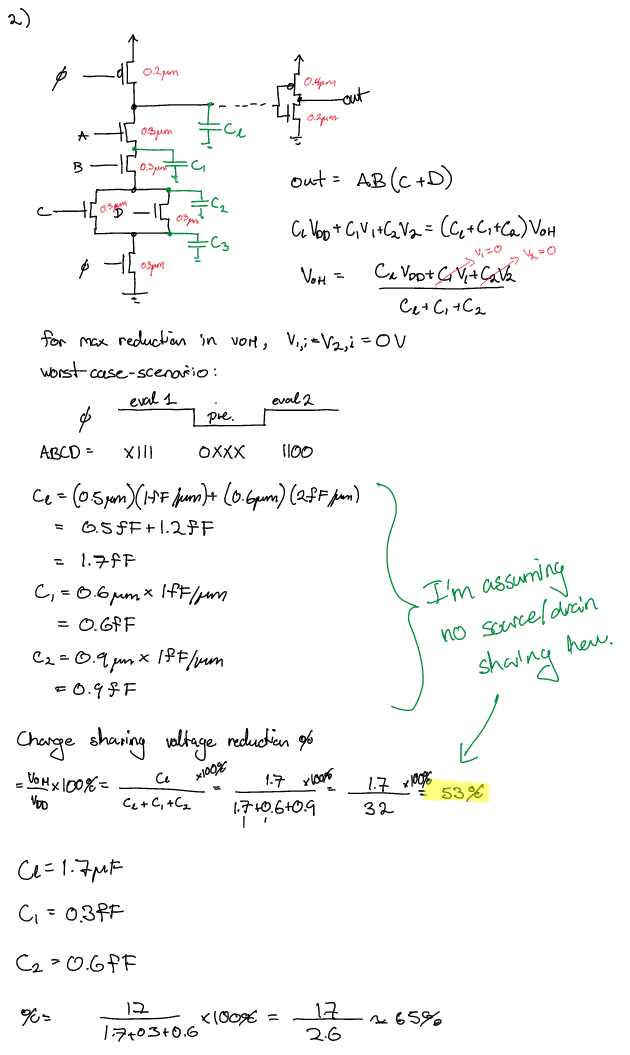
\includegraphics[width=0.8\textwidth]{2a.png}
\end{figure}
\begin{figure}[H]
    \centering
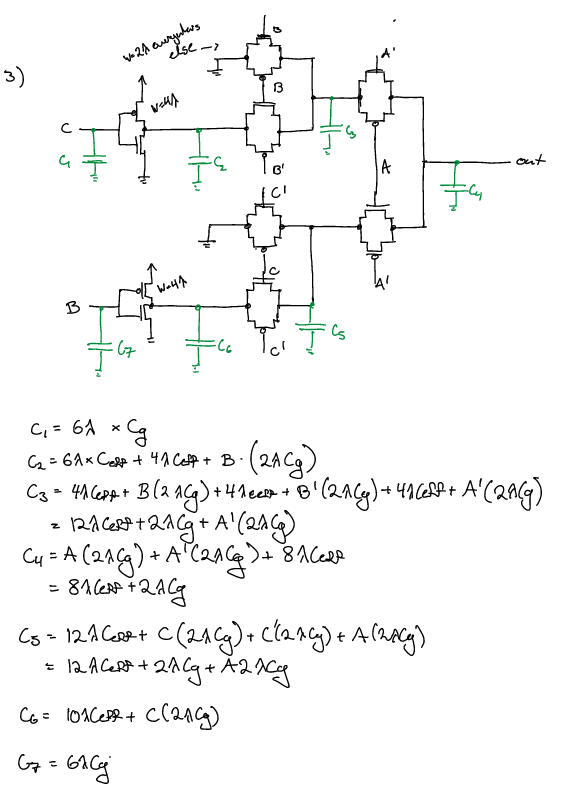
\includegraphics[width=0.8\textwidth]{3a.png}
\end{figure}

\begin{figure}[H]
    \centering
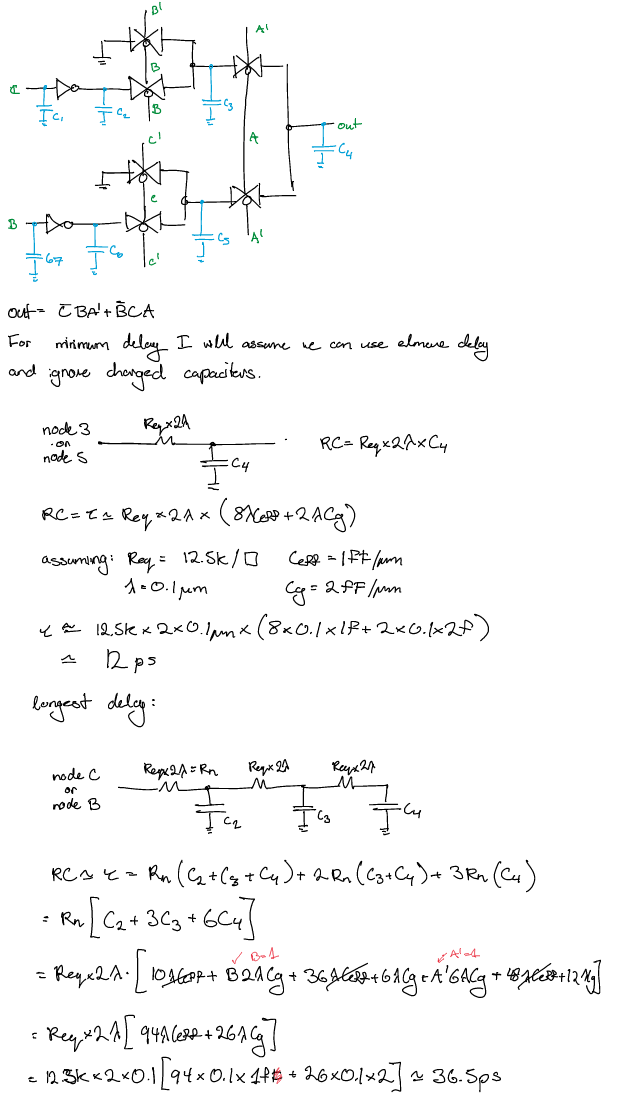
\includegraphics[width=0.8\textwidth]{3b.png}
\end{figure}
\begin{figure}[H]
    \centering
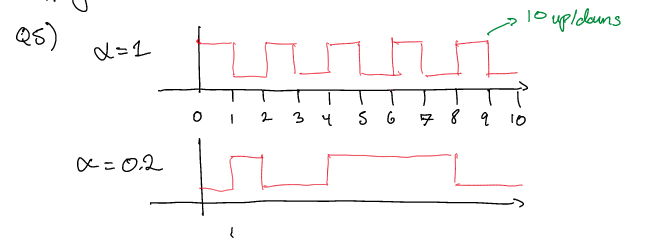
\includegraphics[width=0.8\textwidth]{5.png}
\end{figure}


\end{document}